$\epsilon\!=\!1.0$
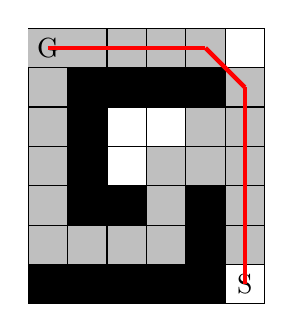
\begin{tikzpicture}[every node/.style={minimum size=.5cm-\pgflinewidth, outer sep=0pt}]
\draw[step=0.5cm,color=black] (-2,-2.5) grid (1,1);
% First row left to right
\node[fill=gray!50] at (-1.75,+0.75) {G};
\node[fill=gray!50] at (-1.25,+0.75) {};
\node[fill=gray!50] at (-0.75,+0.75) {};
\node[fill=gray!50] at (-0.25,+0.75) {};
\node[fill=gray!50] at (+0.25,+0.75) {};
\node at (+0.75,+0.75) {};

% Second row left to right
\node[fill=gray!50] at (-1.75,+0.25) {};
\node[fill=black] at (-1.25,+0.25) {};
\node[fill=black] at (-0.75,+0.25) {};
\node[fill=black] at (-0.25,+0.25) {};
\node[fill=black] at (+0.25,+0.25) {};
\node[fill=gray!50] at (+0.75,+0.25) {};

% Third row left to right
\node[fill=gray!50] at (-1.75,-0.25) {};
\node[fill=black] at (-1.25,-0.25) {};
\node at (-0.75,-0.25) {};
\node at (-0.25,-0.25) {};
\node[fill=gray!50] at (+0.25,-0.25) {};
\node[fill=gray!50] at (+0.75,-0.25) {};

% Fourth row left to right
\node[fill=gray!50] at (-1.75,-0.75) {};
\node[fill=black] at (-1.25,-0.75) {};
\node at (-0.75,-0.75) {};
\node[fill=gray!50] at (-0.25,-0.75) {};
\node[fill=gray!50] at (+0.25,-0.75) {};
\node[fill=gray!50] at (+0.75,-0.75) {};

% Fifth row left to right
\node[fill=gray!50] at (-1.75,-1.25) {};
\node[fill=black] at (-1.25,-1.25) {};
\node[fill=black] at (-0.75,-1.25) {};
\node[fill=gray!50] at (-0.25,-1.25) {};
\node[fill=black] at (+0.25,-1.25) {};
\node[fill=gray!50] at (+0.75,-1.25) {};

% Sixth row left to right
\node[fill=gray!50] at (-1.75,-1.75) {};
\node[fill=gray!50] at (-1.25,-1.75) {};
\node[fill=gray!50] at (-0.75,-1.75) {};
\node[fill=gray!50] at (-0.25,-1.75) {};
\node[fill=black] at (+0.25,-1.75) {};
\node[fill=gray!50] at (+0.75,-1.75) {};

% Seventh row left to right
\node[fill=black] at (-1.75,-2.25) {};
\node[fill=black] at (-1.25,-2.25) {};
\node[fill=black] at (-0.75,-2.25) {};
\node[fill=black] at (-0.25,-2.25) {};
\node[fill=black] at (+0.25,-2.25) {};
\node at (+0.75,-2.25) {S};

% Draw path in red
\draw[ultra thick, red] (-1.75,+0.75) -- (+0.25,+0.75);
\draw[ultra thick, red] (+0.25,+0.75) -- (+0.75,+0.25);
\draw[ultra thick, red] (+0.75,+0.25) -- (+0.75,-2.25);
\end{tikzpicture}
\hspace{0.1cm}
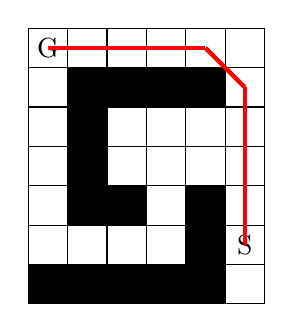
\begin{tikzpicture}[every node/.style={minimum size=.5cm-\pgflinewidth, outer sep=0pt}]
\draw[step=0.5cm,color=black] (-2,-2.5) grid (1,1);
% First row left to right
\node at (-1.75,+0.75) {G};
\node at (-1.25,+0.75) {};
\node at (-0.75,+0.75) {};
\node at (-0.25,+0.75) {};
\node at (+0.25,+0.75) {};
\node at (+0.75,+0.75) {};

% Second row left to right
\node at (-1.75,+0.25) {};
\node[fill=black] at (-1.25,+0.25) {};
\node[fill=black] at (-0.75,+0.25) {};
\node[fill=black] at (-0.25,+0.25) {};
\node[fill=black] at (+0.25,+0.25) {};
\node at (+0.75,+0.25) {};

% Third row left to right
\node at (-1.75,-0.25) {};
\node[fill=black] at (-1.25,-0.25) {};
\node at (-0.75,-0.25) {};
\node at (-0.25,-0.25) {};
\node at (+0.25,-0.25) {};
\node at (+0.75,-0.25) {};

% Fourth row left to right
\node at (-1.75,-0.75) {};
\node[fill=black] at (-1.25,-0.75) {};
\node at (-0.75,-0.75) {};
\node at (-0.25,-0.75) {};
\node at (+0.25,-0.75) {};
\node at (+0.75,-0.75) {};

% Fifth row left to right
\node at (-1.75,-1.25) {};
\node[fill=black] at (-1.25,-1.25) {};
\node[fill=black] at (-0.75,-1.25) {};
\node at (-0.25,-1.25) {};
\node[fill=black] at (+0.25,-1.25) {};
\node at (+0.75,-1.25) {};

% Sixth row left to right
\node at (-1.75,-1.75) {};
\node at (-1.25,-1.75) {};
\node at (-0.75,-1.75) {};
\node at (-0.25,-1.75) {};
\node[fill=black] at (+0.25,-1.75) {};
\node at (+0.75,-1.75) {S};

% Seventh row left to right
\node[fill=black] at (-1.75,-2.25) {};
\node[fill=black] at (-1.25,-2.25) {};
\node[fill=black] at (-0.75,-2.25) {};
\node[fill=black] at (-0.25,-2.25) {};
\node[fill=black] at (+0.25,-2.25) {};
\node at (+0.75,-2.25) {};

% Draw path in blue
\draw[ultra thick, red] (-1.75,+0.75) -- (+0.25,+0.75);
\draw[ultra thick, red] (+0.25,+0.75) -- (+0.75,+0.25);
\draw[ultra thick, red] (+0.75,+0.25) -- (+0.75,-1.75);
\end{tikzpicture}
\hspace{0.1cm}
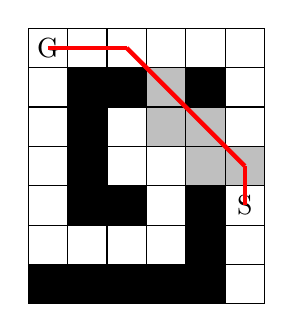
\begin{tikzpicture}[every node/.style={minimum size=.5cm-\pgflinewidth, outer sep=0pt}]
\draw[step=0.5cm,color=black] (-2,-2.5) grid (1,1);
% First row left to right
\node at (-1.75,+0.75) {G};
\node at (-1.25,+0.75) {};
\node at (-0.75,+0.75) {};
\node at (-0.25,+0.75) {};
\node at (+0.25,+0.75) {};
\node at (+0.75,+0.75) {};

% Second row left to right
\node at (-1.75,+0.25) {};
\node[fill=black] at (-1.25,+0.25) {};
\node[fill=black] at (-0.75,+0.25) {};
\node[fill=gray!50] at (-0.25,+0.25) {};
\node[fill=black] at (+0.25,+0.25) {};
\node at (+0.75,+0.25) {};

% Third row left to right
\node at (-1.75,-0.25) {};
\node[fill=black] at (-1.25,-0.25) {};
\node at (-0.75,-0.25) {};
\node[fill=gray!50] at (-0.25,-0.25) {};
\node[fill=gray!50] at (+0.25,-0.25) {};
\node at (+0.75,-0.25) {};

% Fourth row left to right
\node at (-1.75,-0.75) {};
\node[fill=black] at (-1.25,-0.75) {};
\node at (-0.75,-0.75) {};
\node at (-0.25,-0.75) {};
\node[fill=gray!50] at (+0.25,-0.75) {};
\node[fill=gray!50] at (+0.75,-0.75) {};

% Fifth row left to right
\node at (-1.75,-1.25) {};
\node[fill=black] at (-1.25,-1.25) {};
\node[fill=black] at (-0.75,-1.25) {};
\node at (-0.25,-1.25) {};
\node[fill=black] at (+0.25,-1.25) {};
\node at (+0.75,-1.25) {S};

% Sixth row left to right
\node at (-1.75,-1.75) {};
\node at (-1.25,-1.75) {};
\node at (-0.75,-1.75) {};
\node at (-0.25,-1.75) {};
\node[fill=black] at (+0.25,-1.75) {};
\node at (+0.75,-1.75) {};

% Seventh row left to right
\node[fill=black] at (-1.75,-2.25) {};
\node[fill=black] at (-1.25,-2.25) {};
\node[fill=black] at (-0.75,-2.25) {};
\node[fill=black] at (-0.25,-2.25) {};
\node[fill=black] at (+0.25,-2.25) {};
\node at (+0.75,-2.25) {};

% Draw path in blue
\draw[ultra thick, red] (-1.75,+0.75) -- (-0.75,+0.75);
\draw[ultra thick, red] (-0.75,+0.75) -- (+0.75,-0.75);
\draw[ultra thick, red] (+0.75,-0.75) -- (+0.75,-1.25);
\end{tikzpicture}

\vspace*{20px}
$\epsilon\!=\!2.5$
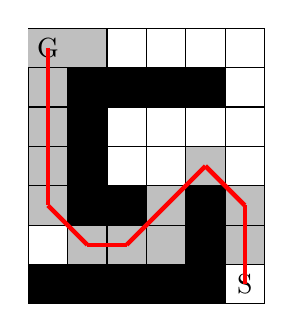
\begin{tikzpicture}[every node/.style={minimum size=.5cm-\pgflinewidth, outer sep=0pt}]
\draw[step=0.5cm,color=black] (-2,-2.5) grid (1,1);
% First row left to right
\node[fill=gray!50] at (-1.75,+0.75) {G};
\node[fill=gray!50] at (-1.25,+0.75) {};
\node at (-0.75,+0.75) {};
\node at (-0.25,+0.75) {};
\node at (+0.25,+0.75) {};
\node at (+0.75,+0.75) {};

% Second row left to right
\node[fill=gray!50] at (-1.75,+0.25) {};
\node[fill=black] at (-1.25,+0.25) {};
\node[fill=black] at (-0.75,+0.25) {};
\node[fill=black] at (-0.25,+0.25) {};
\node[fill=black] at (+0.25,+0.25) {};
\node at (+0.75,+0.25) {};

% Third row left to right
\node[fill=gray!50] at (-1.75,-0.25) {};
\node[fill=black] at (-1.25,-0.25) {};
\node at (-0.75,-0.25) {};
\node at (-0.25,-0.25) {};
\node at (+0.25,-0.25) {};
\node at (+0.75,-0.25) {};

% Fourth row left to right
\node[fill=gray!50] at (-1.75,-0.75) {};
\node[fill=black] at (-1.25,-0.75) {};
\node at (-0.75,-0.75) {};
\node at (-0.25,-0.75) {};
\node[fill=gray!50] at (+0.25,-0.75) {};
\node at (+0.75,-0.75) {};

% Fifth row left to right
\node[fill=gray!50] at (-1.75,-1.25) {};
\node[fill=black] at (-1.25,-1.25) {};
\node[fill=black] at (-0.75,-1.25) {};
\node[fill=gray!50] at (-0.25,-1.25) {};
\node[fill=black] at (+0.25,-1.25) {};
\node[fill=gray!50] at (+0.75,-1.25) {};

% Sixth row left to right
\node at (-1.75,-1.75) {};
\node[fill=gray!50] at (-1.25,-1.75) {};
\node[fill=gray!50] at (-0.75,-1.75) {};
\node[fill=gray!50] at (-0.25,-1.75) {};
\node[fill=black] at (+0.25,-1.75) {};
\node[fill=gray!50] at (+0.75,-1.75) {};

% Seventh row left to right
\node[fill=black] at (-1.75,-2.25) {};
\node[fill=black] at (-1.25,-2.25) {};
\node[fill=black] at (-0.75,-2.25) {};
\node[fill=black] at (-0.25,-2.25) {};
\node[fill=black] at (+0.25,-2.25) {};
\node at (+0.75,-2.25) {S};

% Draw path in red
\draw[ultra thick, red] (-1.75,+0.75) -- (-1.75,-1.25);
\draw[ultra thick, red] (-1.75,-1.25) -- (-1.25,-1.75);
\draw[ultra thick, red] (-1.25,-1.75) -- (-0.75,-1.75);
\draw[ultra thick, red] (-0.75,-1.75) -- (+0.25,-0.75);
\draw[ultra thick, red] (+0.25,-0.75) -- (+0.75,-1.25);
\draw[ultra thick, red] (+0.75,-1.25) -- (+0.75,-2.25);
\end{tikzpicture}
\hspace{0.1cm}
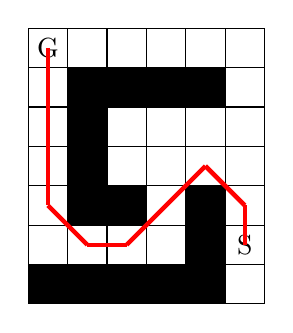
\begin{tikzpicture}[every node/.style={minimum size=.5cm-\pgflinewidth, outer sep=0pt}]
\draw[step=0.5cm,color=black] (-2,-2.5) grid (1,1);
% First row left to right
\node at (-1.75,+0.75) {G};
\node at (-1.25,+0.75) {};
\node at (-0.75,+0.75) {};
\node at (-0.25,+0.75) {};
\node at (+0.25,+0.75) {};
\node at (+0.75,+0.75) {};

% Second row left to right
\node at (-1.75,+0.25) {};
\node[fill=black] at (-1.25,+0.25) {};
\node[fill=black] at (-0.75,+0.25) {};
\node[fill=black] at (-0.25,+0.25) {};
\node[fill=black] at (+0.25,+0.25) {};
\node at (+0.75,+0.25) {};

% Third row left to right
\node at (-1.75,-0.25) {};
\node[fill=black] at (-1.25,-0.25) {};
\node at (-0.75,-0.25) {};
\node at (-0.25,-0.25) {};
\node at (+0.25,-0.25) {};
\node at (+0.75,-0.25) {};

% Fourth row left to right
\node at (-1.75,-0.75) {};
\node[fill=black] at (-1.25,-0.75) {};
\node at (-0.75,-0.75) {};
\node at (-0.25,-0.75) {};
\node at (+0.25,-0.75) {};
\node at (+0.75,-0.75) {};

% Fifth row left to right
\node at (-1.75,-1.25) {};
\node[fill=black] at (-1.25,-1.25) {};
\node[fill=black] at (-0.75,-1.25) {};
\node at (-0.25,-1.25) {};
\node[fill=black] at (+0.25,-1.25) {};
\node at (+0.75,-1.25) {};

% Sixth row left to right
\node at (-1.75,-1.75) {};
\node at (-1.25,-1.75) {};
\node at (-0.75,-1.75) {};
\node at (-0.25,-1.75) {};
\node[fill=black] at (+0.25,-1.75) {};
\node at (+0.75,-1.75) {S};

% Seventh row left to right
\node[fill=black] at (-1.75,-2.25) {};
\node[fill=black] at (-1.25,-2.25) {};
\node[fill=black] at (-0.75,-2.25) {};
\node[fill=black] at (-0.25,-2.25) {};
\node[fill=black] at (+0.25,-2.25) {};
\node at (+0.75,-2.25) {};

% Draw path in red
\draw[ultra thick, red] (-1.75,+0.75) -- (-1.75,-1.25);
\draw[ultra thick, red] (-1.75,-1.25) -- (-1.25,-1.75);
\draw[ultra thick, red] (-1.25,-1.75) -- (-0.75,-1.75);
\draw[ultra thick, red] (-0.75,-1.75) -- (+0.25,-0.75);
\draw[ultra thick, red] (+0.25,-0.75) -- (+0.75,-1.25);
\draw[ultra thick, red] (+0.75,-1.25) -- (+0.75,-1.75);
\end{tikzpicture}
\hspace{0.1cm}
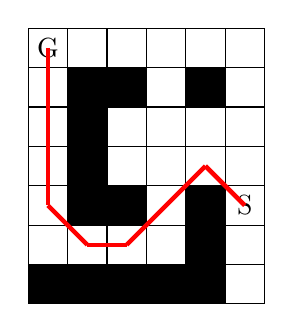
\begin{tikzpicture}[every node/.style={minimum size=.5cm-\pgflinewidth, outer sep=0pt}]
\draw[step=0.5cm,color=black] (-2,-2.5) grid (1,1);
% First row left to right
\node at (-1.75,+0.75) {G};
\node at (-1.25,+0.75) {};
\node at (-0.75,+0.75) {};
\node at (-0.25,+0.75) {};
\node at (+0.25,+0.75) {};
\node at (+0.75,+0.75) {};

% Second row left to right
\node at (-1.75,+0.25) {};
\node[fill=black] at (-1.25,+0.25) {};
\node[fill=black] at (-0.75,+0.25) {};
\node at (-0.25,+0.25) {};
\node[fill=black] at (+0.25,+0.25) {};
\node at (+0.75,+0.25) {};

% Third row left to right
\node at (-1.75,-0.25) {};
\node[fill=black] at (-1.25,-0.25) {};
\node at (-0.75,-0.25) {};
\node at (-0.25,-0.25) {};
\node at (+0.25,-0.25) {};
\node at (+0.75,-0.25) {};

% Fourth row left to right
\node at (-1.75,-0.75) {};
\node[fill=black] at (-1.25,-0.75) {};
\node at (-0.75,-0.75) {};
\node at (-0.25,-0.75) {};
\node at (+0.25,-0.75) {};
\node at (+0.75,-0.75) {};

% Fifth row left to right
\node at (-1.75,-1.25) {};
\node[fill=black] at (-1.25,-1.25) {};
\node[fill=black] at (-0.75,-1.25) {};
\node at (-0.25,-1.25) {};
\node[fill=black] at (+0.25,-1.25) {};
\node at (+0.75,-1.25) {S};

% Sixth row left to right
\node at (-1.75,-1.75) {};
\node at (-1.25,-1.75) {};
\node at (-0.75,-1.75) {};
\node at (-0.25,-1.75) {};
\node[fill=black] at (+0.25,-1.75) {};
\node at (+0.75,-1.75) {};

% Seventh row left to right
\node[fill=black] at (-1.75,-2.25) {};
\node[fill=black] at (-1.25,-2.25) {};
\node[fill=black] at (-0.75,-2.25) {};
\node[fill=black] at (-0.25,-2.25) {};
\node[fill=black] at (+0.25,-2.25) {};
\node at (+0.75,-2.25) {};

% Draw path in red
\draw[ultra thick, red] (-1.75,+0.75) -- (-1.75,-1.25);
\draw[ultra thick, red] (-1.75,-1.25) -- (-1.25,-1.75);
\draw[ultra thick, red] (-1.25,-1.75) -- (-0.75,-1.75);
\draw[ultra thick, red] (-0.75,-1.75) -- (+0.25,-0.75);
\draw[ultra thick, red] (+0.25,-0.75) -- (+0.75,-1.25);
\end{tikzpicture}